\chapter{Nonlinear Difference Equations and Momentum MM}\label{chap:difference}

The two halves of this book meet in a single mathematical object: the
nonlinear difference equation. The Collatz map is one, driven by the parity
of the state. Every first order optimizer is one too, and the momentum\index{momentum}
methods of \cref{chap:momentum} are second order difference equations whose
coefficients may switch with the iteration counter.
This chapter develops the common theory and proves three results, one of them conditionally on a conjecture that we support by computation.

First, the inverse Collatz tree satisfies a system of difference
inequalities, in the spirit of Krasikov\index{Krasikov, I.} and Lagarias\index{Lagarias, J. C.}, from which we derive
and certify explicit growth exponents: for every $n$ not divisible by $3$ and
not on a cycle, at least $c\,X^{0.477}$ integers below $Xn$ have orbits passing
through $n$.
Second, we compute exactly, using a rank one structure, the joint spectral radius\index{joint spectral radius} of the switched linear system that describes Switching MM\index{Switching MM} on a quadratic. It is below one at every parameter value we computed, and if a transient bound that we state as a conjecture holds it is below one for all of them, so that \emph{every} switching rule, including adaptive and state dependent ones, is exponentially stable.
Third, for any $\mu$ strongly convex and $L$ smooth function, not necessarily quadratic, two steps of \smmdet\ contract the distance to the minimizer by an explicit factor, which is the exact worst case over the class: explicit one dimensional functions attain it, and performance estimation\index{performance estimation} confirms it.
This settles open problem S1 of \cref{chap:open} for the distance; for function values the matching bound is exact only above a threshold condition number.
We end with continuous time limits, where a backward error
analysis shows that the implicit regularization\index{implicit regularization} of Switching MM carries the
same Cauchy and Schwarz penalty as its noise floor\index{noise floor}.

\section{The Collatz recursion as a switched system}\label{sec:ch5b:switched}

Write $u_n=\log x_n$ for the logarithm of the $n$th iterate of the accelerated
map $T$. Then
\begin{equation}\label{eq:ch5b:switched}
\begin{gathered}
  u_{n+1}=u_n+g_{b_n}(u_n),\\
  g_0(u)=-\log2,\qquad g_1(u)=\log\Bigl(\tfrac32+\tfrac12e^{-u}\Bigr),
\end{gathered}
\end{equation}
where the switching signal $b_n=x_n\bmod2$ selects one of two vector fields.
In the language of control theory \eqref{eq:ch5b:switched} is a \emph{switched
system} with two modes~\cite{liberzon2003}. Mode $0$ is a constant descent;
mode $1$ is an ascent of size slightly above $\log(3/2)$, larger when $u$ is
small. \Cref{fig:ch5b:switched} shows both branches as traced by real orbits.

Two features distinguish \eqref{eq:ch5b:switched} from the switched systems\index{switched system} of
engineering. The first is that the switching is \emph{state dependent} in an
arithmetic, not a geometric, way: $b_n$ is a function of $x_n=e^{u_n}$, but
of its parity, which changes on scales of size $e^{-u_n}$ in $u$. The second
is that the system is unstable under \emph{arbitrary} switching: the signal
$b_n\equiv1$ gives $u_n\ge u_0+n\log(3/2)$. Stability, if it holds, must come
from the particular signal the arithmetic produces. The following elementary
statement makes the threshold precise.

\begin{proposition}[The switching frequency decides]\label{prop:ch5b:freq}
Let $p_N$ be the proportion of odd steps among the first $N$ steps of the
orbit of $x_0$ under $T$. Then
\begin{align*}
  N\bigl(p_N\log3-\log2\bigr)&\le u_N-u_0\\
  &\le N\bigl(p_N\log3-\log2\bigr)+\sum_{n<N,\ b_n=1}\frac{1}{3x_n}.
\end{align*}
In particular an orbit along which $\liminf_Np_N>1/\lt=0.6309$ is unbounded,
and an orbit along which $\limsup_Np_N<1/\lt-1/(3Y\log3)$ cannot stay above $Y$ at every step.
\end{proposition}

\begin{proof}
Each odd step contributes $\log(3/2+1/(2x_n))=\log(3/2)+\log(1+1/(3x_n))$,
which lies between $\log(3/2)$ and $\log(3/2)+1/(3x_n)$, and each even step
contributes $-\log2$. Summing, $u_N-u_0$ lies between
$Np_N\log(3/2)-N(1-p_N)\log2=N(p_N\log3-\log2)$ and that quantity plus
$\sum1/(3x_n)$ over the odd steps. The first consequence follows from the lower
bound. For the second, if $x_n\ge Y$ for all $n$ then the correction is at most
$Np_N/(3Y)\le N/(3Y)$, and the upper bound tends to $-\infty$ under the stated
condition, contradicting $x_n\ge Y$.
\end{proof}

The proposition is the Ces\`aro identity\index{Cesaro identity@Ces\`aro identity} of \cref{chap:divergence} written for
$T$ rather than for the Syracuse map\index{Syracuse map}: the threshold $1/\lt$ for the proportion
of odd steps corresponds to the threshold $\lt$ for halvings per odd step. In
the language of switched systems, the divergence half of the conjecture asserts that the state
dependent switching signal never dwells in mode $1$ with frequency at or above
$1/\lt$ for long.
\Cref{thm:nolyapunov} and \cref{cor:ch4:multistride} say that no strictly increasing function of $x$ decreases along every stride, an odd step together with the halvings that follow it, nor along every block of $J$ strides for any fixed $J$, so no such function, used as a Lyapunov function\index{Lyapunov function}, can certify this; the certificate\index{certificate}, if there is one, must read the arithmetic of the signal (\cref{rem:ch4:monotone}).

\begin{figure}[ht]
\centering
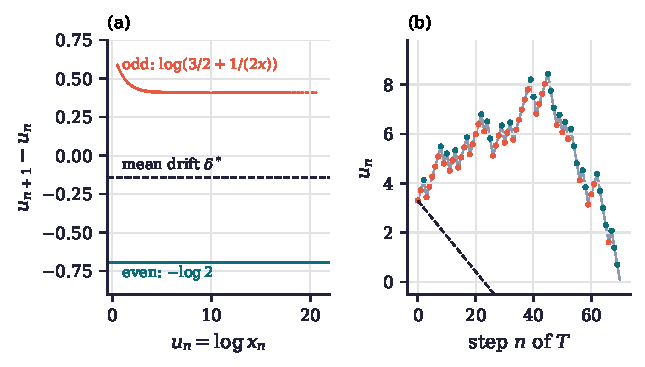
\includegraphics[width=\textwidth]{figures/ch5b_switched.pdf}
\caption{The Collatz recursion as a switched system in $u=\log x$. (a) Increments $u_{n+1}-u_n$ against $u_n$ along $60$ orbits started between $10^6$ and $10^7$; odd steps follow the curve $\log(3/2+1/(2x))$, even steps the constant $-\log2$, and the dashed line is the mean drift $\ds=\log(\sqrt3/2)$ of the Bernoulli model. (b) The orbit of $27$ under $T$, shaded by mode, with the drift line $\log27+n\ds$; every odd step rises and every even step falls.}
\label{fig:ch5b:switched}
\end{figure}

\section{Difference inequalities for the inverse tree}\label{sec:ch5b:tree}

The deepest unconditional lower bounds on how many integers reach $1$ come
from a different difference equation, one satisfied by counting functions on
the inverse tree\index{inverse tree}. Krasikov\index{Krasikov, I.}~\cite{krasikov1989} introduced the method, obtaining
the exponent $3/7$ from a system of inequalities modulo $9$; Applegate\index{Applegate, D.} and
Lagarias\index{Lagarias, J. C.}~\cite{applegate1995} reached $0.81$ by solving larger systems with
linear programming, and Krasikov and Lagarias~\cite{krasikov2003} enlarged the
systems further and reached the exponent $0.84$: for large $x$, at least
$x^{0.84}$ integers up to $x$ have orbits that reach $1$. We develop a simple
version of the method here, complete with proofs, which already gives an
exponent above $3/7$ and shows clearly where the difference inequalities\index{difference inequality} come
from. Accounts of the full method are in~\cite{krasikov2003,lagarias2010}.

\paragraph{The inverse tree.} Under $T$ every $n$ has the preimage $2n$, and
also the preimage $(2n-1)/3$ when $n\equiv2\pmod3$. Starting from a root $n$,
the \emph{doubling chain} $n,2n,4n,\dots$ lies in its inverse tree, and an
element $p=2^jn$ of the chain with $j\ge1$ has the odd preimage
\[
  c_j(n)=\frac{2^{j+1}n-1}{3}\qquad\text{when }2^jn\equiv2\pmod 3.
\]
If moreover $2^jn\equiv2$ or $8\pmod9$, then $c_j(n)\not\equiv0\pmod3$ and
$c_j(n)$ has odd preimages of its own; we call such $j$ \emph{fertile}. For
$n\not\equiv0\pmod3$ let
\[
  \pi_n(X)=\#\{m\le Xn:\ \text{the orbit of }m\text{ under }T\text{ passes through }n\}.
\]

\begin{lemma}[Difference inequality]\label{lem:ch5b:diffineq}
Let $n\not\equiv0\pmod3$ be an integer that does not lie on a cycle of $T$.
Then for every $X\ge1$,
\begin{equation}\label{eq:ch5b:diffineq}
  \pi_n(X)\;\ge\;\sum_{j\ \mathrm{fertile},\ 2^{j+1}\le3X}
  \pi_{c_j(n)}\Bigl(\frac{3X}{2^{j+1}}\Bigr).
\end{equation}
\end{lemma}

\begin{proof}
If $m$ is counted in $\pi_{c_j}(3X/2^{j+1})$ then its orbit passes through $c_j$,
hence through $T(c_j)=2^jn$ and then through $n$, and
$m\le(3X/2^{j+1})c_j=Xn-X/2^{j+1}<Xn$. So each term counts integers that are
also counted by $\pi_n(X)$. The sets for different fertile $j$ are disjoint:
the orbit of $m$ reaches $n$ for the first time along a unique path, which
passes through exactly one element of the doubling chain immediately after an
odd step, namely $2^jn=T(c_j)$; since $n$ is not on a cycle, the orbit cannot
reach $n$, leave it, and return through another branch.
\end{proof}

The inequality \eqref{eq:ch5b:diffineq} is a difference inequality, linear in the counting functions,
in the scale variable $\log X$: it bounds a counting function at scale $X$ by
the same family of functions at the smaller scales $3X/2^{j+1}$, with an index
$c_j(n)$ that moves through residue classes. The residue class of $c_j(n)$
modulo $3^k$ is determined by $n\bmod3^{k+1}$ and $j\bmod2\cdot3^k$, the period
of $2$ modulo $3^{k+1}$. This suggests a power law ansatz with a constant
depending on the class.

\begin{theorem}[Certified growth exponents]\label{thm:ch5b:exponent}
Fix $k\ge1$ and let $\mathcal R_k$ be the residues modulo $3^k$ prime to $3$.
For $g>0$ and a positive vector $(w_r)_{r\in\mathcal R_k}$ define
\[
  (\Phi_g w)_r=\min_{\ell}\ \sum_{j\ \mathrm{fertile\ for}\ \ell}
  \Bigl(\frac3{2^{j+1}}\Bigr)^g w_{[c_j(\ell)]},
\]
where the minimum is over the three lifts $\ell$ of $r$ to residues modulo
$3^{k+1}$, fertility and the class $[c_j(\ell)]\in\mathcal R_k$ depend only on
$\ell$ and $j$, and the sum is over all $j\ge1$. If $\Phi_g w\ge(1+\eta)w$
componentwise for some $\eta>0$, then there is $C>0$ such that
\[
  \pi_n(X)\;\ge\;C\,w_{[n]}\,X^g\qquad\text{for all }X\ge1
\]
and all $n\not\equiv0\pmod3$ not lying on a cycle of $T$.
\end{theorem}

\begin{proof}
The sum defining $\Phi_g$ converges, since its terms decay like $2^{-jg}$; by
the periodicity of the classes in $j$ it equals the sum over one period times
$1/(1-2^{-Pg})$ with $P=2\cdot3^k$. The terms with $2^{j+1}>3X$, which are
missing from \eqref{eq:ch5b:diffineq}, have total weight at most
$w_{\max}\sum_{2^{j+1}>3X}(3/2^{j+1})^g\le w_{\max}X^{-g}/(1-2^{-g})$,
which is below $\eta\,w_{\min}$ once $X\ge X_0$ for a suitable $X_0$. Choose
$C=1/(w_{\max}X_0^g)$, so that the claim holds for $X\le X_0$ because
$\pi_n(X)\ge1$ (the root itself is counted). For $X>X_0$ argue by strong induction
on the scale: every argument $3X/2^{j+1}$ in \eqref{eq:ch5b:diffineq} is at most
$3X/4<X$, and the children $c_j(n)$ are again prime to $3$ and not on a cycle
(an element of a cycle has its image on the cycle, and $T(c_j)=2^jn$ leads to
$n$). Hence
\begin{align*}
  \pi_n(X)&\ge C X^g\sum_{\substack{j\ \mathrm{fertile}\\2^{j+1}\le3X}}
  \Bigl(\frac3{2^{j+1}}\Bigr)^g w_{[c_j(n)]}\\
  &\ge CX^g\bigl((1+\eta)w_{[n]}-\eta w_{\min}\bigr)\ge CX^g w_{[n]},
\end{align*}
using that the full sum is at least $(\Phi_g w)_{[n]}$, because the lift of
$[n]$ determined by $n\bmod3^{k+1}$ is one of the three in the minimum.
\end{proof}

The theorem reduces a lower bound for an infinite family of counting
functions to a finite eigenvalue problem: find the largest $g$ for which the
monotone, homogeneous operator $\Phi_g$, nonlinear only through the minimum over lifts, has a positive supersolution. We solved
it by power iteration and bisection in $g$, and certified each exponent by
exhibiting a vector $w$ with $\min_r(\Phi_g w)_r/w_r>1$ (script
\texttt{ch5b\_tree.py}), and checked each certificate in exact integer arithmetic, with every power of $2$ and $3$ rounded down (script \texttt{ch5b\_tree\_exact.py}). The results are
\[
\begin{array}{c|cccccc}
k & 2 & 3 & 4 & 5 & 6 & 7\\\hline
\text{classes} & 6 & 18 & 54 & 162 & 486 & 1458\\
\gamma_k & 0.416 & 0.435 & 0.449 & 0.460 & 0.470 & 0.477
\end{array}
\]
with certified margins $1+\eta$ between $1.0002$ and $1.0027$.
The certificate for $k=7$ still has margin $1.0001$ at $g=0.47705$, so for the root $n=4$, which reaches $1$ and is not on a cycle, the theorem gives $\pi_4(X)\ge c\,X^{0.47705}$ for some $c>0$, which exceeds $(4X)^{0.477}$ for all large $X$. This gives the following.

\begin{corollary}[A counting bound]\label{cor:ch5b:count}
For all large $x$, at least $x^{0.477}$ integers $m\le x$ have orbits that
reach $1$.
\end{corollary}

The exponents increase with the modulus but slowly, and they are bounded by
what single doubling chains can produce. A mean field heuristic predicts the
limit. On average one third of the $j$ are fertile, and if the class constants
were all equal the supersolution condition would read
$\tfrac13\sum_{j\ge1}(3/2^{j+1})^g=1$, that is $3^{g-1}=2^g(2^g-1)$, whose root
is $g=0.4927$.
The exact counts of the doubling chain construction approach it: for roots $n=4,5,7$ the number of integers it generates below $Xn$ grows with exponent $0.500$, $0.502$ and $0.498$ over the last decade of $X$ up to $2^{20}$, and with exponent $0.492$, $0.494$ and $0.492$ over the last decade up to $2^{36}$ (script \texttt{ch5b\_chains.py}), while the true counting functions $\pi_n(X)$ grow with exponent $1.000$ (\cref{fig:ch5b:tree}).
The gap between $1/2$ and $0.84$ comes from a branch that the doubling chain system leaves out. Every element $p\equiv2\pmod3$ of the inverse tree has the odd preimage $(2p-1)/3<p$, the term $j=0$; seen from $p$, its count enters at the larger scale $3X/2$, so the induction on scale in the proof of \cref{thm:ch5b:exponent} cannot use it. With this branch the mean field equation becomes $\tfrac13\sum_{j\ge0}(3/2^{j+1})^g=1$, that is $3^{g-1}=2^g-1$, whose smaller root is exactly $g=1$. Krasikov's inequalities keep these terms, which Krasikov and Lagarias call advanced; Applegate and Lagarias truncated them to reach $0.81$, and Krasikov and Lagarias reached $0.84$ by proving that the linear programming bounds remain valid with the advanced terms present~\cite{krasikov2003}. The elements divisible by $3$ play no role: such an element has no odd preimage, so its inverse tree is a single doubling chain. The gap between $0.84$ and $1$ is open.
The exponent $1$ would already follow from a positive
proportion of integers reaching $1$, which is far short of the conjecture.

\begin{figure}[ht]
\centering
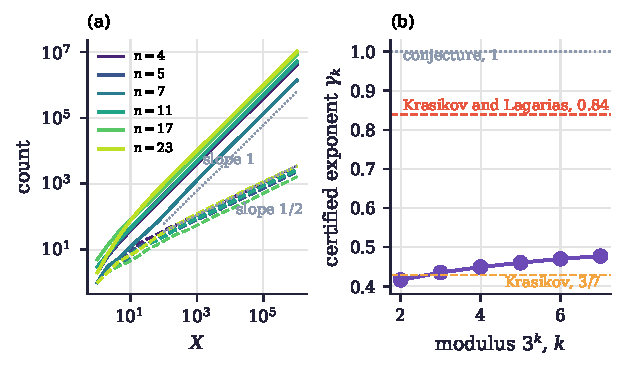
\includegraphics[width=\textwidth]{figures/ch5b_tree.pdf}
\caption{(a) Exact counting functions $\pi_n(X)$ (solid) and the counts produced
by the doubling chain construction (dashed) for several roots $n$, up to
$X=2^{20}$; the true counts grow linearly, the construction roughly like $X^{1/2}$. (b)
Certified exponents $\gamma_k$ from \cref{thm:ch5b:exponent} for moduli $3^k$,
against Krasikov's $3/7$, the exponent $0.84$ of Krasikov and Lagarias, and the
conjectured value $1$.}
\label{fig:ch5b:tree}
\end{figure}

\section{Momentum MM as a difference equation}\label{sec:ch5b:mm}

We now turn to the optimizers. For an $L$ smooth function $f$ the descent lemma
says that
\begin{equation}\label{eq:ch5b:major}
  f(y)\le Q_L(y\mid x):=f(x)+\langle\nabla f(x),y-x\rangle+\tfrac L2\|y-x\|^2
\end{equation}
for all $x,y$, with equality at $y=x$. So $Q_L(\cdot\mid x)$ majorizes $f$ in the
sense of \cref{chap:lyapunov}, and its minimizer is the gradient step
$G_{1/L}(x)=x-\nabla f(x)/L$. Gradient descent is the MM algorithm\index{MM algorithm} for this
majorizer\index{majorization}, and the MM descent property gives
$f(G_{1/L}(x))\le f(x)-\|\nabla f(x)\|^2/(2L)$.

Momentum methods of Nesterov's type majorize at a different point. Given an \emph{anchor}
$y_t=x_t+\beta_t(x_t-x_{t-1})$, they set $x_{t+1}=\arg\min_yQ_L(y\mid y_t)
=G_{1/L}(y_t)$. With $\beta_t\equiv\beta$ this is Nesterov's method; with
$\beta_t=\beta$ for odd $t$ and $\beta_t=0$ for even $t$ it is \smmdet. We call
the general scheme \emph{momentum\index{momentum} MM}: an MM iteration whose majorization point
is extrapolated on a schedule. Written out, it is the second order nonlinear
difference equation
\begin{equation}\label{eq:ch5b:momentummm}
  x_{t+1}=F_t(x_t,x_{t-1}):=y_t-\tfrac1L\nabla f(y_t),\qquad
  y_t=x_t+\beta_t(x_t-x_{t-1}),
\end{equation}
which is periodic in $t$ for Switching MM\index{Switching MM} and autonomous for Nesterov\index{Nesterov acceleration}.

Momentum MM gives up the monotonicity of MM: Nesterov's method, like heavy ball\index{heavy ball},
is not a descent method, and its function values oscillate. Switching MM
keeps it on alternate iterates, for every smooth function, convex or not.

\begin{proposition}[Monotonicity on alternate iterates]\label{prop:ch5b:monotone}
Let $f$ be $L$ smooth and bounded below by $f_{\inf}$, and run \smmdet\ with
step $1/L$ and $\beta\in[0,1)$. For even $t$,
\[
  f(x_{t+2})\le f(x_t)-\frac{1-\beta^2}{2L}\|\nabla f(x_t)\|^2
  -\frac1{2L}\|\nabla f(y_{t+1})\|^2 .
\]
Consequently $\min_{t<2K,\ t\ \mathrm{even}}\|\nabla f(x_t)\|^2\le
2L(f(x_0)-f_{\inf})/((1-\beta^2)K)$.
\end{proposition}

\begin{proof}
By \cref{lem:ch6:ystep}, $y_{t+1}=G_{(1+\beta)/L}(x_t)$ and
$x_{t+2}=G_{1/L}(y_{t+1})$. For a gradient step of length $h$ the descent lemma
gives $f(G_h(x))\le f(x)-h(1-Lh/2)\|\nabla f(x)\|^2$. With $h=(1+\beta)/L$ the
coefficient is $(1+\beta)(1-\beta)/(2L)$, and with $h=1/L$ it is $1/(2L)$. Adding
the two inequalities gives the first claim, and summing over $K$ periods gives
the second.
\end{proof}

The extrapolation is safe because it is a gradient step of length
$(1+\beta)/L<2/L$, inside the range where the descent lemma still guarantees
decrease. Momentum at every step has no such interpretation: its anchor
carries the whole history of past gradients.

\section{Stability theory}\label{sec:ch5b:stability}

\subsection{Lyapunov functions for difference equations}

A function $V\ge0$ is a Lyapunov function\index{Lyapunov function} for the difference equation
$z_{t+1}=F_t(z_t)$ with rate $\rho<1$ if $V(z_{t+1})\le\rho V(z_t)$ for all $t$
and $z_t$; then $V(z_t)\le\rho^tV(z_0)$. For gradient descent on a $\mu$ strongly
convex, $L$ smooth function, $V=f-f^*$ works with $\rho=1-1/\kappa$. For
Nesterov\index{Nesterov acceleration}'s method with constant momentum\index{momentum} $\beta=(\sqrt\kappa-1)/(\sqrt\kappa+1)$
and step $1/L$, Nesterov\index{Nesterov, Yu.}'s estimate sequence construction gives the Lyapunov
function $f(x_t)-f^*+\frac\mu2\|v_t-x^*\|^2$, with $v_t$ an auxiliary sequence that
is an affine combination of $x_t$ and $x_{t-1}$, and the rate
$1-1/\sqrt\kappa$: for every $t$,
\[
  f(x_t)-f^*\le\Bigl(1-\frac1{\sqrt\kappa}\Bigr)^t\Bigl(f(x_0)-f^*
  +\frac\mu2\|x_0-x^*\|^2\Bigr),
\]
see~\cite{nesterov2004}, and~\cite{wilson2021} for the Lyapunov reading.
The point to retain is that the Lyapunov function of an accelerated method must involve two consecutive iterates, because the state of the method is the pair $(x_t,x_{t-1})$: started at $x_t=x^*$ with $x_{t-1}\ne x^*$ the method in general leaves the minimizer, so no function of $x_t$ alone that vanishes only at $x^*$ can decrease at every step.

\subsection{Switching and the joint spectral radius}

On one eigendirection of a quadratic, with $a=\alpha\lambda$ and state
$z_t=(e_t,e_{t-1})$, the two steps of \smmdet\ are the matrices
\[
  D=\begin{pmatrix}1-a&0\\1&0\end{pmatrix},\qquad
  N=\begin{pmatrix}(1-a)(1+\beta)&-(1-a)\beta\\1&0\end{pmatrix},
\]
for a descent and an injection respectively. \smmdet\ applies them in the
periodic order $D,N,D,N,\dots$, every step Nesterov\index{Nesterov acceleration} applies $N$ always, and the
adaptive rule \smmstate\ of \cref{chap:smm} applies them in an order that depends on the state.
What can be said for an \emph{arbitrary} order? The relevant quantity is the
joint spectral radius\index{joint spectral radius} of Rota\index{Rota, G. C.} and Strang\index{Strang, G.}~\cite{rota1960},
\[
  \hat\rho(\{D,N\})=\lim_{k\to\infty}\max_{M_i\in\{D,N\}}
  \|M_k\cdots M_1\|^{1/k},
\]
which is the best possible exponential rate valid for every switching sequence;
see~\cite{jungers2009} for the theory. It is in general hard to compute. Here it
is not, because $D$ has rank one.

\begin{proposition}[Exact joint spectral radius]\label{prop:ch5b:jsr}
Write $D=vu^\top$ with $u=(1,0)^\top$ and $v=(1-a,1)^\top$, and put
$\tau_j=u^\top N^jv$, the first coordinate after $j$ injections started from
the state left by one descent step. Then
\[
  \hat\rho(\{D,N\})=\max\Bigl(\rho(N),\ \sup_{j\ge0}|\tau_j|^{1/(j+1)}\Bigr).
\]
\end{proposition}

\begin{proof}
By the theorem of Berger\index{Berger, M. A.} and Wang\index{Wang, Y.} (see~\cite{jungers2009}) the joint spectral
radius equals $\limsup_k\max\rho(M_k\cdots M_1)^{1/k}$ over products, and by
cyclic invariance of the spectrum it suffices to consider products that are
either $N^k$ or begin with $D$. A product beginning with $D$ is, up to cyclic
permutation, $DN^{j_1}DN^{j_2}\cdots DN^{j_m}$ with $\sum(j_i+1)=k$. Since
$D=vu^\top$, this product equals $v\,\bigl(\prod_{i}u^\top N^{j_i}v\bigr)$ times
$u^\top$ in the appropriate order, a rank one matrix with the single nonzero
eigenvalue $\prod_i\tau_{j_i}$. Hence $\rho^{1/k}=\prod_i|\tau_{j_i}|^{1/k}\le
\max_i|\tau_{j_i}|^{1/(j_i+1)}$, with equality when all $j_i$ are equal. Taking
the supremum over products gives the formula.
\end{proof}

The formula needs only the scalar sequence $\tau_j$, which tends to zero
geometrically at rate $\rho(N)<1$, so the maximum in the formula is attained, at a finite $j$ or by $\rho(N)$,
and can be computed to any accuracy (script \texttt{ch5b\_jsr.py}). The result
is striking (\cref{fig:ch5b:jsr}). For every $a$ we computed the joint spectral
radius is below $1$, and it exceeds the larger of the two pure rates, $\max(\rho(D),
\rho(N))$, by at most $0.0056$ at $\beta=\lt-1$ and $0.0011$ at $\beta=0.9$, over
a grid of $400$ values of $a$ from $10^{-4}$ to $0.999$. For small $a$ it equals
$1-a$, the rate of gradient descent, attained by the product $D$ alone.

Since $\tau_j\to0$, the joint spectral radius is below $1$ exactly when
$|\tau_j|<1$ for every $j$.
Over a grid of $200$ values of $\beta\in[0,0.999]$ and $300$ values of $a\in[10^{-5},0.9999]$ we found $\sup_j|\tau_j|=\tau_0=1-a$ in every case, with a quadratic Lyapunov function of $N$ bounding the terms beyond those computed (script \texttt{ch5b\_transient.py}): the transient of the injection steps never exceeds the first descent.
We record this as a conjecture.

\begin{conjecture}[Transient bound]\label{conj:ch5b:transient}
For all $a\in(0,1]$, $\beta\in[0,1)$ and $j\ge0$, $|\tau_j|\le1-a$.
\end{conjecture}

Note that while $e$ stays positive the bound is immediate: with
$d_t=e_{t-1}-e_t$ one has $e_{t+1}=(1-a)(e_t-\beta d_t)$ and
$d_{t+1}=ae_t+(1-a)\beta d_t$, with $e_0=1-a$ and $d_0=a$. As long as $e$ stays
nonnegative, $d$ stays nonnegative and $e_{t+1}\le(1-a)e_t$, so $e$ decreases
and $|e_t|\le1-a$. The difficulty is the oscillating regime after $e$ changes
sign.

\begin{corollary}[Every switching rule is stable]\label{cor:ch5b:anyswitch}
Fix $a\in(0,1)$ and suppose $|\tau_j|<1$ for all $j$, as
\cref{conj:ch5b:transient} asserts and as computation confirms on the grid
above. Then on a quadratic with spectrum in $(0,L]$ and step $1/L$, every
switching sequence between descent and injection steps, whether periodic,
random, or chosen adaptively from the state as in \smmstate, converges to the
minimizer on the eigendirection with $a=\alpha\lambda$, with exponential rate at
most $\hat\rho(\{D(a),N(a)\})<1$.
\end{corollary}

This is partial progress on open problem S4 of \cref{chap:open}. At every grid point above, and for all $a$ and $\beta$ if \cref{conj:ch5b:transient} holds, adaptive switching cannot destabilize the method. On the grid of $400$ values of $a$ it also cannot make the contraction factor more than $0.0056$ larger than that of the worse of gradient descent and every step Nesterov at $\beta=\lt-1$, which is about one percent per step and $1.8$ percent in the number of iterations, and at $\beta=0.9$ the cost is $0.12$ percent per step and $1.1$ percent in iterations. Stability alone does not close the noiseless gap to every step momentum that S4 asks about.
The Collatz switched system\index{switched system} \eqref{eq:ch5b:switched} is the opposite case: there
the joint behaviour under arbitrary switching is unstable, and all the
difficulty lies in the switching signal.

\begin{figure}[ht]
\centering
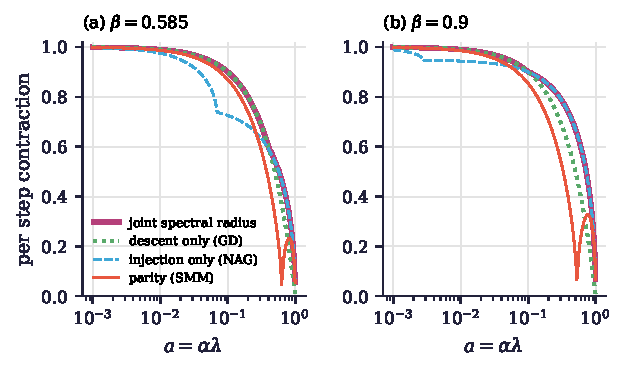
\includegraphics[width=\textwidth]{figures/ch5b_jsr.pdf}
\caption{The joint spectral radius of the descent and injection matrices,
computed exactly by \cref{prop:ch5b:jsr}, against $a=\alpha\lambda$, together
with the per step rates of pure descent (gradient descent), pure injection
(every step Nesterov) and the parity schedule of \smmdet. The joint spectral
radius hugs the upper envelope of the two pure rates.}
\label{fig:ch5b:jsr}
\end{figure}

\section{A linear rate beyond quadratics}\label{sec:ch5b:rate}

\Cref{thm:smmquad} described \smmdet\ exactly on quadratics. For a general
smooth strongly convex function the same identity, \cref{lem:ch6:ystep}, holds
with no change, and it reduces the convergence question to the classical
contraction of a single gradient step.

\begin{theorem}[Linear rate of \smmdet]\label{thm:ch5b:rate}
Let $f$ be $\mu$ strongly convex and $L$ smooth with minimizer $x^*$, put
$\kappa=L/\mu$, and run \smmdet\ with step $\alpha=1/L$ and $\beta\in[0,1)$. For
every even $t$,
\begin{gather*}
  \|x_{t+2}-x^*\|\le q\,\|x_t-x^*\|,\\
  q=q(\beta,\kappa)=\Bigl(1-\frac1\kappa\Bigr)\max\Bigl(1-\frac{1+\beta}\kappa,\
  \beta\Bigr),
\end{gather*}
and $f(x_{t+2})-f^*\le q^2\,(f(x_t)-f^*)$.
\end{theorem}

\begin{proof}
By \cref{lem:ch6:ystep}, $x_{t+2}=G_{1/L}(G_{(1+\beta)/L}(x_t))$. For a step
$h\in(0,2/L)$ and $f$ twice differentiable,
$G_h(x)-x^*=x-x^*-h(\nabla f(x)-\nabla f(x^*))=(I-h\bar H)(x-x^*)$ with
$\bar H=\int_0^1\nabla^2f(x^*+s(x-x^*))\,ds$, whose eigenvalues lie in
$[\mu,L]$. Hence $\|G_h(x)-x^*\|\le\max(|1-h\mu|,|1-hL|)\|x-x^*\|$; for $f$ that
is only once differentiable the same bound follows by smoothing, or directly
from the cocoercivity of $\nabla f$. With $h=(1+\beta)/L$ the factor is
$\max(1-(1+\beta)/\kappa,\beta)$, and with $h=1/L$ it is $1-1/\kappa$. Composing
gives the distance bound.
For function values, Taylor\index{Taylor, A. B.}, Hendrickx\index{Hendrickx, J. M.} and Glineur\index{Glineur, F.}~\cite[Theorem~3.3]{taylor2018} show that a gradient step of length $h\in(0,2/L)$ satisfies $f(G_h(x))-f^*\le\max((1-h\mu)^2,(1-hL)^2)(f(x)-f^*)$; composing the two steps gives the second bound.
\end{proof}

How good is this? The contraction of each gradient step is tight for the class,
so one might worry only about the composition. We computed the exact worst case
of two steps of \smmdet\ over all $\mu$ strongly convex, $L$ smooth functions in
every dimension by \emph{performance estimation\index{performance estimation}}~\cite{drori2014,taylor2017}: the
worst case is the value of a small semidefinite program built from the
interpolation conditions of the class (script \texttt{ch5b\_pep.py}). For
$\beta\in\{0.3,\lt-1,0.9\}$ and $\kappa\in\{2,3,5,10,20,50,100\}$ the worst case
of $\|x_{t+2}-x^*\|^2/\|x_t-x^*\|^2$ agreed with $q^2$ to six digits in all $21$
cases.
So the distance bound of \cref{thm:ch5b:rate} is the exact worst case, not merely a bound, and explicit functions attain it for every $\kappa$. When $\kappa\ge(1+\beta)/(1-\beta)$, which is $\kappa\ge3.82$ at $\beta=\lt-1$, both factors are attained at the eigenvalue $\mu$ and the worst case is the quadratic $\frac\mu2\|x\|^2$. For smaller $\kappa$ the two factors are attained at different curvatures, and the worst function is not quadratic: the one dimensional function equal to $\frac L2x^2$ for $x\ge0$ and to $\frac\mu2x^2$ for $x<0$ attains $q$, since from $x_t=1$ the long step lands at $-\beta$ and the short step at $-\beta(1-1/\kappa)$.
The function value bound $q^2$ is exact only for $\kappa\ge(1+\beta)/(1-\beta)$, where the same quadratic attains it. Below that threshold performance estimation for function values gives a smaller worst case, for example $0.049$ against $q^2=0.086$ at $\beta=\lt-1$ and $\kappa=2$.

\begin{corollary}[Speed relative to gradient descent]\label{cor:ch5b:speed}
For $\kappa\ge(1+\beta)/(1-\beta)$ the per step rate of \smmdet\ is
$q^{1/2}=((1-1/\kappa)(1-(1+\beta)/\kappa))^{1/2}$, so that
$-\kappa\log q^{1/2}\to(2+\beta)/2$ as $\kappa\to\infty$, against $1$ for gradient
descent with the same step. This is the effective step multiplier of
\cref{cor:ch6:slow}, now valid on the whole class.
\end{corollary}

\Cref{fig:ch5b:rate} plots the normalized rate $-\kappa\log q/2$ against $\kappa$.
It lies below gradient descent exactly when $\kappa<1/(1-\beta)$, which is $\kappa<2.41$ at $\beta=\lt-1$: there the long step $(1+\beta)/L$ overshoots the large curvatures and the factor $\beta$ dominates. On the range of the figure it is largest at $\kappa=(1+\beta)/(1-\beta)$, where the two factors of $q$ balance ($1.60$ at $\beta=\lt-1$), and beyond that point it decreases to $(2+\beta)/2$, which is $1.29$ at $\beta=\lt-1$, as $\kappa\to\infty$.
Open problem S1 asked for exactly this:
a linear rate on the whole class with the constant predicted by the quadratic
analysis. The answer is that the quadratic constant is exact for $\kappa\ge(1+\beta)/(1-\beta)$, and in particular as $\kappa\to\infty$.

\begin{figure}[ht]
\centering
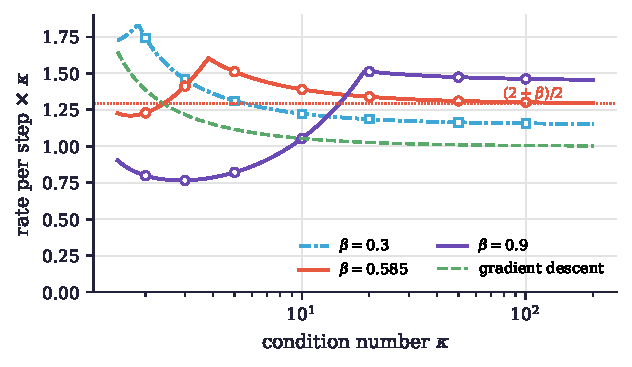
\includegraphics[width=\textwidth]{figures/ch5b_rate.pdf}
\caption{Worst case per step rate of \smmdet\ for the distance to the minimizer on the class of $\mu$ strongly
convex, $L$ smooth functions, multiplied by $\kappa$, from
\cref{thm:ch5b:rate} (lines) and from performance estimation (open markers), for
three values of $\beta$; gradient descent with step $1/L$ is dashed. At large
$\kappa$ the normalized rate of \smmdet\ tends to $(2+\beta)/2$.}
\label{fig:ch5b:rate}
\end{figure}

\section{Continuous time limits}\label{sec:ch5b:ode}

The continuous time view of \cref{chap:momentum} describes accelerated methods by
second order differential equations, obtained by letting the step size tend to
zero while the momentum\index{momentum} tends to one at a matched rate: for heavy ball\index{heavy ball} with
step $s$ and $\beta=1-c\sqrt s$, the limit is the damped oscillator
$\ddot x+c\dot x+\nabla f(x)=0$ on the time scale $t=k\sqrt s$, and Nesterov\index{Nesterov acceleration}'s
method with $\beta_k=(k-1)/(k+2)$ gives the equation of Su\index{Su, W.}, Boyd\index{Boyd, S.} and
Cand\`es\index{Candes, E. J.@Cand\`es, E. J.}~\cite{su2016}. With $\beta$ \emph{fixed} and $\alpha\to0$ the picture is
different, and it is the relevant one for a fixed default such as
$\beta=\lt-1$.

\begin{proposition}[Modified equation for period two steps]\label{prop:ch5b:modified}
Let $f$ be three times differentiable and consider the composition of gradient
steps of lengths $h_1$ and $h_2$, in either order. To second order in
$h=h_1+h_2$ it agrees with the time $h$ flow of the modified equation\index{modified equation}
\begin{equation}\label{eq:ch5b:modified}
\begin{aligned}
  \dot x&=-\nabla f(x)-\frac{h_1^2+h_2^2}{2(h_1+h_2)}\,\nabla^2f(x)\nabla f(x)\\
  &=-\nabla\Bigl(f+\frac{\bar h}{4}\|\nabla f\|^2\Bigr),\qquad
  \bar h=\frac{h_1^2+h_2^2}{h_1+h_2}.
\end{aligned}
\end{equation}
\end{proposition}

\begin{proof}
Write $g=\nabla f$ and $H=\nabla^2f$. Expanding,
$G_{h_2}(G_{h_1}(x))=x-h_1g-h_2g(x-h_1g)+O(h^3)=x-hg+h_1h_2Hg+O(h^3)$, and the
term $h_1h_2Hg$ is symmetric in the two steps. The time $h$ flow of
$\dot x=-g-cHg$ is $x-hg-hcHg+\frac{h^2}2Hg+O(h^3)$, because the second
derivative of the flow is $Hg$ to leading order. Matching the coefficients of
$Hg$ gives $-hc+h^2/2=h_1h_2$, so $c=(h^2/2-h_1h_2)/h=(h_1^2+h_2^2)/(2h)$. Finally
$Hg=\nabla(\frac12\|g\|^2)$.
\end{proof}

For a single gradient step of length $h$ the same computation gives the
modified function $f+\frac h4\|\nabla f\|^2$, the implicit gradient
regularization of Barrett\index{Barrett, D. G. T.} and Dherin\index{Dherin, B.}~\cite{barrett2021}; backward error analysis
of this kind is classical in geometric numerical
integration~\cite{hairer2006}. For \smmdet, $h_1=(1+\beta)\alpha$ and
$h_2=\alpha$, so the iteration follows the gradient flow of
\[
  f+\frac{\alpha V(\beta)}{4}\|\nabla f\|^2,\qquad
  V(\beta)=\frac{(1+\beta)^2+1}{2+\beta},
\]
on the time scale $(2+\beta)\alpha/2$ per iteration; $V(\beta)$ is the slow mode noise amplification of \cref{cor:ch7:slow}. Two conclusions follow.

First, Switching MM\index{Switching MM} has no inertial limit. Whatever the value of $\beta<1$, its
continuous time limit is a first order gradient flow, sped up by the factor
$(2+\beta)/2$ and implicitly regularized. This is the continuous counterpart of
\cref{rem:ch6:reframing}: the method carries one gradient of memory, not a
velocity, and no rescaling turns it into a damped oscillator.

Second, the implicit regularization\index{implicit regularization} strength has a familiar ratio. Gradient
descent run at the same speed, with step $(2+\beta)\alpha/2$, has regularization
coefficient $(2+\beta)\alpha/8$, while \smmdet\ has $V(\beta)\alpha/4$. Their
ratio is
\[
  \frac{2V(\beta)}{2+\beta}=\frac{2\bigl((1+\beta)^2+1\bigr)}{(2+\beta)^2}
  =1+\frac{\beta^2}{(2+\beta)^2},
\]
exactly the noise floor\index{noise floor} penalty of \cref{prop:ch7:matched} and of the gain weight\index{gain weight theorem}
theorem, \cref{thm:ch7:gainweight}. This is not a coincidence. Both quantities are the ratio of the mean
square step to the square of the mean step, $\frac12(h_1^2+h_2^2)/
(\frac12(h_1+h_2))^2$, which Cauchy and Schwarz bounds below by $1$. Unequal steps
cost the same factor whether one measures the stationary noise or the implicit
bias.

\section*{Notes}

The stability of switched systems\index{switched system} under arbitrary and constrained switching
is surveyed by Liberzon\index{Liberzon, D.}~\cite{liberzon2003}; the joint spectral radius\index{joint spectral radius} is due to
Rota and Strang~\cite{rota1960}, and Jungers\index{Jungers, R.}~\cite{jungers2009} covers both
its computation and the theorem of Berger and Wang. The difference inequality\index{difference inequality} method
for the inverse Collatz tree is due to Krasikov\index{Krasikov, I.}~\cite{krasikov1989}, with
improvements by Applegate and Lagarias\index{Lagarias, J. C.}~\cite{applegate1995} and the sharpest
results by Krasikov and Lagarias~\cite{krasikov2003}; the survey volume~\cite{lagarias2010}
gives the history. The doubling chain system, \cref{thm:ch5b:exponent} and its
certified exponents are our simplified version and are far from the state of
the art. The view of gradient descent as an MM algorithm\index{MM algorithm} through the descent
lemma is standard~\cite{lange2000,hunter2004}; the name momentum\index{momentum} MM, the
monotonicity and joint spectral radius propositions, and the rate theorem are
ours, with the
function value step bound taken from Taylor, Hendrickx and
Glineur~\cite{taylor2018}.
For finite sets of rank one matrices, Ahmadi\index{Ahmadi, A. A.} and Parrilo\index{Parrilo, P. A.}~\cite{ahmadi2012} reduce the joint spectral radius in the same way to products around cycles, a maximum cycle mean problem; \cref{prop:ch5b:jsr}, with one matrix of rank one, is a variant of their device.
Performance estimation was introduced by Drori\index{Drori, Y.} and
Teboulle\index{Teboulle, M.}~\cite{drori2014} and made exact for smooth strongly convex functions by
Taylor, Hendrickx and Glineur~\cite{taylor2017}. Modified equations and backward
error analysis are treated in~\cite{hairer2006}, and their use for implicit
regularization in~\cite{barrett2021}.

\section*{Exercises}

\begin{exercise}
Show that under arbitrary switching the system \eqref{eq:ch5b:switched} can realize every sequence of modes, that while $u_n\ge0$ every increment lies in $\{-\log2\}\cup(\log\frac32,\log2]$, and that a run of mode $1$ increments is strictly decreasing. Show also that for the actual Collatz signal no two consecutive steps of the standard map\index{standard map} $T_0$ are odd.
What does this say about the
frequencies achievable under $T_0$?
\end{exercise}

\begin{exercise}
Compute by hand the operator $\Phi_g$ of \cref{thm:ch5b:exponent} for $k=1$,
with classes $1,2\bmod3$ and lifts modulo $9$, and find the largest $g$ for
which it has a positive supersolution. Compare with the values in the table.
\end{exercise}

\begin{exercise}
Verify the mean field equation $3^{g-1}=2^g(2^g-1)$ and show that it has a
unique root in $(0,1)$. Explain why the doubling chain construction cannot give
an exponent above this root for typical roots.
\end{exercise}

\begin{exercise}
Show that \cref{prop:ch5b:monotone} fails for every step heavy ball\index{heavy ball}: construct
an $L$ smooth convex quadratic in one dimension and a starting point for which
$f(x_{t+2})>f(x_t)$ for some even $t$ with $\beta=0.585$ and step $1/L$.
\end{exercise}

\begin{exercise}
Compute $\tau_0,\tau_1,\tau_2$ of \cref{prop:ch5b:jsr} in closed form and
show that $|\tau_1|^{1/2}$ is the per step rate of the periodic schedule. For
which $a$ does the supremum in the proposition occur at $j=0$?
\end{exercise}

\begin{exercise}
Using \cref{thm:ch5b:rate}, find the value of $\beta$ that minimizes $q(\beta,\kappa)$
for a given $\kappa$, and show that it tends to $1$ as $\kappa\to\infty$. Compare
the resulting rate with gradient descent and with Nesterov\index{Nesterov acceleration}'s optimal
$1-1/\sqrt\kappa$.
\end{exercise}
